\titledquestion{Topological Sort}

    Given the following DAG, run topological sort with a queue. Write down the vertex you select and update the in-degree \texttt{ind[i]} of all vertices in each iteration.  
	
	\textit{Note: When pushing several vertices into the queue at the same time, push them alphabetically. You are NOT required to show your queue at each step.}
	
	\vspace{1cm}

	\begin{figure}[htbp]
		\centering
		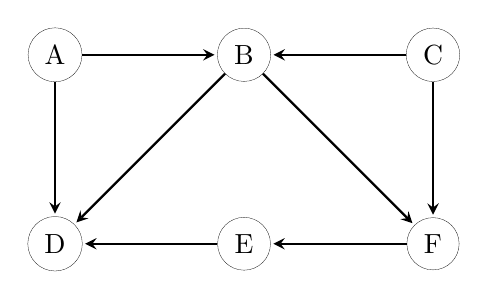
\begin{tikzpicture}[
			> = stealth, % arrow head style
			shorten > = 1pt, % don't touch arrow head to node
			node distance = 1cm, % distance between nodes
			thick, % line style
			scale = 0.8,
		]
		\node[circle, draw, line width=0.1pt] (a) at (-3,3){A};
		\node[circle, draw, line width=0.1pt] (b) at (0, 3){B};
		\node[circle, draw, line width=0.1pt] (c) at (3, 3){C};
		\node[circle, draw, line width=0.1pt] (d) at (-3,0){D};
		\node[circle, draw, line width=0.1pt] (e) at (0, 0){E};
		\node[circle, draw, line width=0.1pt] (f) at (3, 0){F};
		\draw[->] (a) to (b);
		\draw[->] (a) to (d);
		\draw[->] (b) to (d);
		\draw[->] (b) to (f);
		\draw[->] (c) to (b);
		\draw[->] (c) to (f);
		\draw[->] (f) to (e);
		\draw[->] (e) to (d);
		\end{tikzpicture}
	\end{figure}
	\vspace{0.5cm}

	\begin{table}[htbp]
		\begin{center}  
			\begin{tabular}{|l|c|l|l|l|l|l|l|}  
				\hline  
				 & vertex & \texttt{ind[A]} & \texttt{ind[B]} & \texttt{ind[C]} & \texttt{ind[D]} & \texttt{ind[E]} & \texttt{ind[F]}\\ \hline  
				initial     & / & 0  & 2  & 0  & 3  &  1 & 2  \\ \hline    
				iteration 1 & A  & 0  & 1  & 0  & 2  & 1  & 2  \\ \hline    
				iteration 2 & C  & 0  & 0  & 0  & 2  & 1  & 1  \\ \hline    
				iteration 3 & B  & 0  & 0  & 0  & 1  & 1  & 0  \\ \hline    
				iteration 4 & F  & 0  & 0  & 0  & 1  & 0  & 0  \\ \hline   
				iteration 5 & E  & 0  & 0  & 0  & 0  & 0  & 0  \\ \hline    
				iteration 6 & D  & 0  & 0  & 0  & 0  & 0  & 0  \\ 
				\hline  
			\end{tabular}  
		\end{center}
	\end{table}
	\vspace{0.5cm}



\begin{parts}
    \part[5] I. Fill in the table above. II. What is the topological sorting that you obtain?
    \begin{solution}
        %%%%%%%%%%%%%%%%%%%%%%%%%%%%%%%%%%%%%%%%%%%%%%%%%
        % Replace `\vspace{2in}' with your answer.
        %\vspace{1in}
        \\$A,C,B,F,E,D$
		%%%%%%%%%%%%%%%%%%%%%%%%%%%%%%%%%%%%%%%%%%%%%%%%%
    \end{solution}
    \part[3] How many different topological sortings does this graph have? Write them down.
    \begin{solution}
        %%%%%%%%%%%%%%%%%%%%%%%%%%%%%%%%%%%%%%%%%%%%%%%%%
        % Replace `\vspace{2in}' with your answer.
        %\vspace{1in}
        \\2
		\\$A,C,B,F,E,D$
		\\$C,A,B,F,E,D$
		%%%%%%%%%%%%%%%%%%%%%%%%%%%%%%%%%%%%%%%%%%%%%%%%%
    \end{solution}
\end{parts}